\section{Zielsetzung}
In den beiden folgenden Experimenten soll die Ablenkung von Elektronen im elektrischen und magnetischen Feld untersucht werden. Außerdem soll die Stärke des Erdmagnetfeldes und die spezifische Masse eines Elektrons bestimmt werden und zu letzt soll die Empfindlichkeit einer Kathodenstrahlröhre untersucht werden.

\section{Theoretische Grundlage}
\label{sec:Theorie}
\subsection{Aufbau der Kathodenstrahlröhre}
Die beiden Versuche werden in einem evakuierten Glasbehälter durchgeführt, da die Elektronen sonst mit den Luftmolekülen wechselwirken würden. Dazu wird die Kathodenstrahlröhre (Braunsche Röhre) verwendet. Diese besteht aus drei Hauptkomponenten: der Elektronenkanone, einem Ablenksystem und einem Nachweissystem.\\
\textbf{Die Elektronenkanone} erzeugt freie Elektronen durch Glühemission und beschleunigt diese. Dazu wird ein Kathode indirekt beheizt und von dem Wehnelt-Zylinder umgeben. Mit diesem kann die Intensität des Elektronenstrahls gesteuert werden. Die Elektronen werden durch die nachfolgenden Elektroden beschleunigt und fokussiert. \\
\textbf{Das Ablenksystem} besteht aus zwei, zueinander parallelen Kondensatorplatten, welche ein annähernd homogenes elektrisches Feld erzeugen in dem die Elektronen abgelenkt werden. \\
\textbf{Das Nachweissystem} ist ein Leuchtschirm, welcher den auftrefenden Elektronenstrahl visualisiert.\\
In der Abbildung \eqref{fig:Kathode} wird der Sachverhalt verdeutlicht.

\begin{figure}[H]
	\centering
	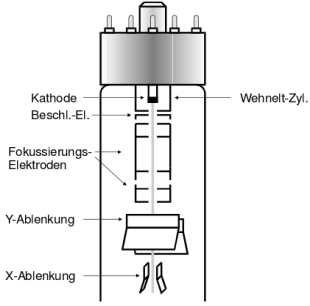
\includegraphics[height=6.5cm]{picture/Kathodenstrahlroehre.PNG}
	\caption{Schematischer Aufbau einer Kathodenstrahlröhre. \cite[2]{V501}}
	\label{fig:Kathode}
\end{figure}

\subsection{Ablenkung von Elektronen im E-Feld}
Zwischen der Glühkathode und den Beschleunigerelektroden liegt eine hohe Spannung $U_\text{B}$ an, sodass die Elektronen beschleunigt werden. Aus der Energieerhaltung folgt:
\begin{equation}
	\frac{m_0 v^2}{2} = e_0 U_\text{B}
\end{equation}
mit der Elementarladung $e_0$, der Elektronenmasse $m_0$ und der Geschwindigkeit $v$. \\
Durch das ändern der Kondensatorspannung wird die Ablenkung des Elektronenstrahls vergrößert oder verkleinert. Diese Ablenkung hängt von der Feldstärke $E$ und der Elektronengeschwindigkeit $v$ ab. Außerdem wird angenommen, dass der Plattenabstand $d$ viel kleiner als die Plattenlänge $p$ ist, somit gilt:
\begin{align*}
	E = \frac{U_\text{d}}{d}
\end{align*}
wobei $U_\text{d}$ der Ablenkspannung entspricht. \\
Unter Betrachtung der Geschwindigkeitskomponenten, dem Winkel $\theta$ der Richtungsänderung und der Abbildung \eqref{fig:AblenkungE} ergibt sich für die Verschiebung $D$:
\begin{equation}
	D = L\theta = \frac{p L U_\text{d}}{2 d U_\text{B}}
	\label{eqn:DUd}
\end{equation}
Mit dem Abstand $L$ zwischen Kondensator und Nachweissystem. \\

\begin{figure}[H]
	\centering
	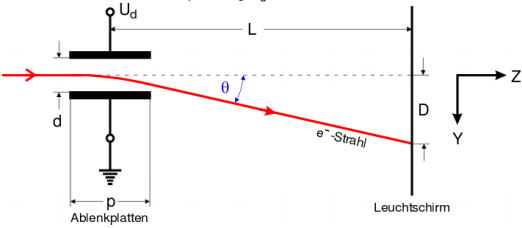
\includegraphics[height=6.5cm]{picture/AblenkungEFeld}
	\caption{Die Ablenkung eines Elektronenstrahls im E-Feld. \cite[3]{V501}}
	\label{fig:AblenkungE}
\end{figure}

Um genaue Messergebnisse erzielen zu können müssen daher $L$ und $p$ möglichst groß und $U_\text{B}$ möglichst klein gewählt werden. Allerdings können an einer solchen Röhre nur Wechselspannungen mit kleiner Frequenz untersucht werden. Um Wechselspannungen mit hoher Frequenz zu untersuchen muss eine Kathodenstrahlröhre mit kleinem $p$ und großem $U_\text{B}$ gewählt werden.

\subsection{Ablenkung von Elektronen im B-Feld}
Im Gegensatz zum elektrischen Feld, wirken in magnetische Felder nur Kräfte auf relativ zum Feld bewegte Ladungen. Diese Kraft wird Lorentz-Kraft $\vec{F}_\text{L}$ genannt.
\begin{equation}
	\vec{F}_\text{L} = q \ \vec{v} \times \vec{B}
	\label{eqn:FL}
\end{equation}
Mit der Ladung $q$, der Geschwindigkeit $\vec{v}$ und dem Magnetfeld $\vec{B}$.\\
Es wird also nur eine Kraft auf die Ladung ausgeübt wenn es eine Geschwindigkeitskomponente senkrecht zum Magnetfeld gibt. Wenn nun ein Elektron, mit konstanter Geschwindigkeit $v_0$, senkrecht in ein homogenes Magnetfeld fliegt, wird das Elektron senkrecht zu $\vec{v}$ und $\vec{B}$ abgelenkt. Nach der Lorentz-Kraft aus Gleichung \eqref{eqn:FL} steht diese in jedem Bahnpunkt senkrecht zum Wegelemt $d \vec{s}$. Mit diesen Überlegungen und dem Kräftegleichgewicht von Lorentz-Kraft und Zentrifugalkraft ergibt sich der Krümmungsradius $r$ zu:
\begin{equation}
	r = \frac{m_0 v_0}{e_0 B}
	\label{eqn:r}
\end{equation}
Mit $e_0$ als Elementarladung und $m_0$ als Elektronenmasse. Die Zentrifugalkraft ist gleich
\begin{align*}
	\frac{m_0\, v^2}{r} \ .
\end{align*}

\begin{figure}[H]
	\centering
	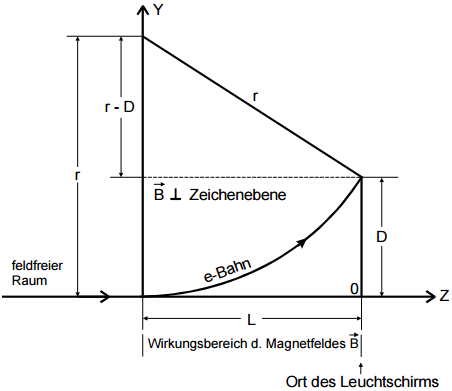
\includegraphics[height=7cm]{picture/AblenkungBFeld}
	\caption{Die Ablenkung eines Elektronenstrahls im B-Feld. \cite[2]{V502}}
	\label{fig:AblenkungB}
\end{figure}

Mit $v_0 = \sqrt{2 U_\text{B} \frac{e_0}{m_0}}$ und der Abbildung \eqref{fig:AblenkungB} folgt die Bestimmungsgleichung für die Ladung eines Elektrons zu:
\begin{equation}
	\frac{D}{L^2 + D^2} = \frac{1}{\sqrt{8 U_\text{B}}} \sqrt{\frac{e_0}{m_0}} B
	\label{eqn:e0m}
\end{equation}
Mit der Verschiebung $D$ und dem Wirkungsbereich $L$ des Magnetfeldes.

\subsection{Magnetfeld einer Helmholtzspule}
Eine Helmholtzspule wird oft verwendet wenn ein annähernd homogenes Magnetfeld benötigt wird. Sie besteht aus zwei Ringspulen, mit jeweils dem Radius $R$ und der Windungszahl $N$, welche parallel zueinander aufgebaut sind. Das Magnetfeld einer Helmholtzspule lässt sich aus
\begin{center}
	\begin{align}
		B = \mu_0 \frac{8}{\sqrt{125}} \frac{N I}{R}
		\label{eqn:BH}
	\end{align}
	\small{(I = \text{Spulenstrom}, $\mu_0$ = \text{Magnetische Feldkonstante})}
\end{center}
berechnen.

\subsection{Erdmagnetfeld}
Die Erde besitzt ein Magnetfeld, welches vom geographischen Südpol zum Nordpol verläuft. Der Winkel unter welchem die magnetischen Feldlinien in die Erdoberfläche eintreten wird als Inklinationswinkel bezeichnet.

\subsection{Fehlerrechnung}
Sämtliche Fehlerrechnungen werden mit Hilfe des Paketes "uncertainties" von Python 3.4.3 durchgeführt.
\subsubsection{Mittelwert}
Der Mittelwert einer Messreihe $x_\text{1}, ... ,x_\text{n}$ lässt sich durch die Formel
\begin{equation}
	\overline{x} = \frac{1}{N} \sum_{\text{k}=1}^\text{N} x_k
	\label{eqn:ave}
\end{equation}
berechnen. Die Standardabweichung des Mittelwertes beträgt
\begin{equation}
	\Delta \overline{x} = \sqrt{ \frac{1}{N(N-1)} \sum_{\text{k}=1}^\text{N} (x_\text{k} - \overline{x})^2}
	\label{eqn:std}
\end{equation}

\subsubsection{Gauß'sche Fehlerfortpflanzung}
Wenn $x_\text{1}, ..., x_\text{n}$ fehlerbehaftete Messgrößen im weiteren Verlauf benutzt werden, wird der neue Fehler $\Delta f$ mit Hilfe der Gaußschen Fehlerfortpflanzung angegeben.
\begin{equation}
	\Delta f = \sqrt{\sum_{\text{k}=1}^\text{N} \left( \frac{ \partial f}{\partial x_\text{k}} \right) ^2 \cdot (\Delta x_\text{k})^2}
	\label{eqn:var}
\end{equation}

\subsubsection{Regression}
Sämtliche Regressionen werden mit Hilfe der Funktion $"scipy.optimize.curve_fit"$ ausgeführt.
